\chapter{Understanding LSTM Locomotion Mode Recognition Behaviour}
\label{chp:lstm-general}

\section{Introduction and Commentary}
% Where possible please ensure that the page numbers tie in with the rest of the thesis document, 
% where this is not possible, you should insert an extra page before the academic paper which shows 
% the citation details and gives the page numbers of the thesis that the academic paper covers.
A large issue identified in literature was the lack of performance classification of novel unseen subjects. To address this research gap further work is required on understanding what prevents \acrshort{lstm} networks from correctly classifying novel subjects.

The \acrshort{lstm} network was selected as HAR is a time-series classification problem with, where input data that are close in space may be dependent while distant sequence of samples in time are assumed as independent. Rae et al.~showed that the \acrshort{lstm} networks adjust well to subject-specific variations\cite{Rai2019}. Thus, the LSTM is renowned for its performance on \acrshort{lmr} tasks\cite{Ordonez2016, Cheng2019, Pienaar2019} 

Following the data collection, work began on developing a general-purpose \acrfull{lstm} network for classifying the locomotive mode of a previously unseen user. This involved work to understand how LSTM networks can recognise different locomotive modes. Once completed, an article entitled ``Understanding LSTM Network Behaviour of IMU-Based Locomotion Mode Recognition for Applications in Prostheses and Wearables'' was submitted to the Journal Sensors. The paper was submitted as part of a call for papers on Machine Learning and Multimodal Sensing for Smart Wearable Assistive Robotics and published on the 10\textsuperscript{th} of February 2021.

The remainder of this chapter will be the presentation of the paper, followed by a short post-commentary. The paper is re-typeset to match the thesis. Page, section and reference numbering has been changed from the published copy.

%\newcommand\x{\value{page}}
 %The paper is presented as published and as such contains both the journal and thesis page numbering. The full paper covers thesis pages \the\numexpr\x+2\relax \ to \the\numexpr\x+24\relax.


\section*{Authorship and permissions}
% \newcommand{\backgoundColor}{0.871,0.918,0.965}
\newcommand{\backgoundColor}{1,1,1}
\newcommand{\boxColor}{0.95,0.95,0.95}
\begin{table}[H]
\caption{Statement of Authorship}
\hyphenpenalty=10000
\begin{tabularx}{\textwidth}{>{\raggedright}p{1.5in}X}
\hline
\rowcolor[rgb]{\backgoundColor}
\multicolumn{2}{l}{\textbf{This declaration concerns the article entitled:}}\\
\hline
\multicolumn{2}{p{0.9\textwidth}}{Understanding LSTM Network Behaviour of IMU-Based Locomotion Mode Recognition for Applications in Prostheses and Wearables} \\

\hline
\rowcolor[rgb]{\backgoundColor}
\multicolumn{2}{l}{\textbf{Publication status (tick one)}}  \\
\rowcolor[rgb]{\backgoundColor}
\multicolumn{2}{l}{\begin{tabular}{rcrcrcrcrc}
    \textbf\ {Draft} &{\cellcolor[rgb]{\boxColor}} \ &
    \textbf{\ Submitted} &{\cellcolor[rgb]{\boxColor}} \ &
    \textbf{\ In review} &{\cellcolor[rgb]{\boxColor}} \ &
    \textbf{\ Accepted} &{\cellcolor[rgb]{\boxColor}} \ &
    \textbf{\ Published} &{\cellcolor[rgb]{\boxColor}}X 
\end{tabular}}  \\
\rowcolor[rgb]{\backgoundColor}\multicolumn{2}{l}{} \\

% Publication details
\hline
{\cellcolor[rgb]{\backgoundColor}}\textbf{Publication details (reference)} & Sensors 2021, 21, 1264.

DOI: \href{https://doi.org/10.3390/s21041264}{10.3390/s21041264} 

Received: 23 December 2020, Accepted: 6 February 2021, Published: 10 February 2021\\


\hline
\rowcolor[rgb]{\backgoundColor}
\multicolumn{2}{l}{\textbf{Publication status (tick one)}} 

\\
\rowcolor[rgb]{\backgoundColor}
\multicolumn{2}{l}{\begin{tabular}{rcrc}
    \textbf{I hold the copyright} &{\cellcolor[rgb]{\boxColor}} \ &
    \textbf{\ Copyright is retained by the publisher, but} &{\cellcolor[rgb]{\boxColor}}X \\
    \textbf{for this material}& & \textbf{I have been given permission to replicate} & \\
    & & \textbf{ the material here} & \\
\end{tabular}}  \\
\rowcolor[rgb]{\backgoundColor}\multicolumn{2}{l}{} \\

\hline
{\cellcolor[rgb]{\backgoundColor}}\textbf{Candidate’s contribution to the paper (provide details, and also indicate as a percentage)} & The candidate predominantly executed the:

\textbf{Formulation of ideas: (95\%)}

The experiment and analysis methodology was conceived by Freddie Sherratt with supervision from Pejman Iravani

\textbf{Design of methodology: (95\%)}

The experiment and analysis methodology was conceived by Freddie Sherratt with supervision from Pejman Iravani

\textbf{Experimental work: (95\%)}

The experimental work was carried out entirely by Freddie Sherratt with supervision from Pejman Iravani

\textbf{Presentation of data in journal format: (95\%)}

The data presentation was carried out entirely by Freddie Sherratt with supervision from Pejman Iravani and Andrew Plummer\\

\hline
{\cellcolor[rgb]{\backgoundColor}}\textbf{Statement from Candidate} &
This paper reports on original research I conducted during the period of my Higher Degree by Research candidature.\\

\hline
{\cellcolor[rgb]{\backgoundColor}}\textbf{Signed} & Freddie Sherratt 
{\begin{tabular}{p{0.6in}ll}
     \ & {\cellcolor[rgb]{\backgoundColor}}\textbf{\ \ Date } & 4th March 2021 
\end{tabular}}\\
\hline
\end{tabularx}
\end{table}
\clearpage

% Paper
% \phantomsection
% \addtocounter{section}{1}
% \addcontentsline{toc}{section}{\arabic{chapter}.\arabic{section}~~~ Article: Understanding LSTM Network Behaviour of IMU-Based Locomotion Mode Recognition  for Applications in Prostheses and Wearables}

% This is the published PDF copy
% 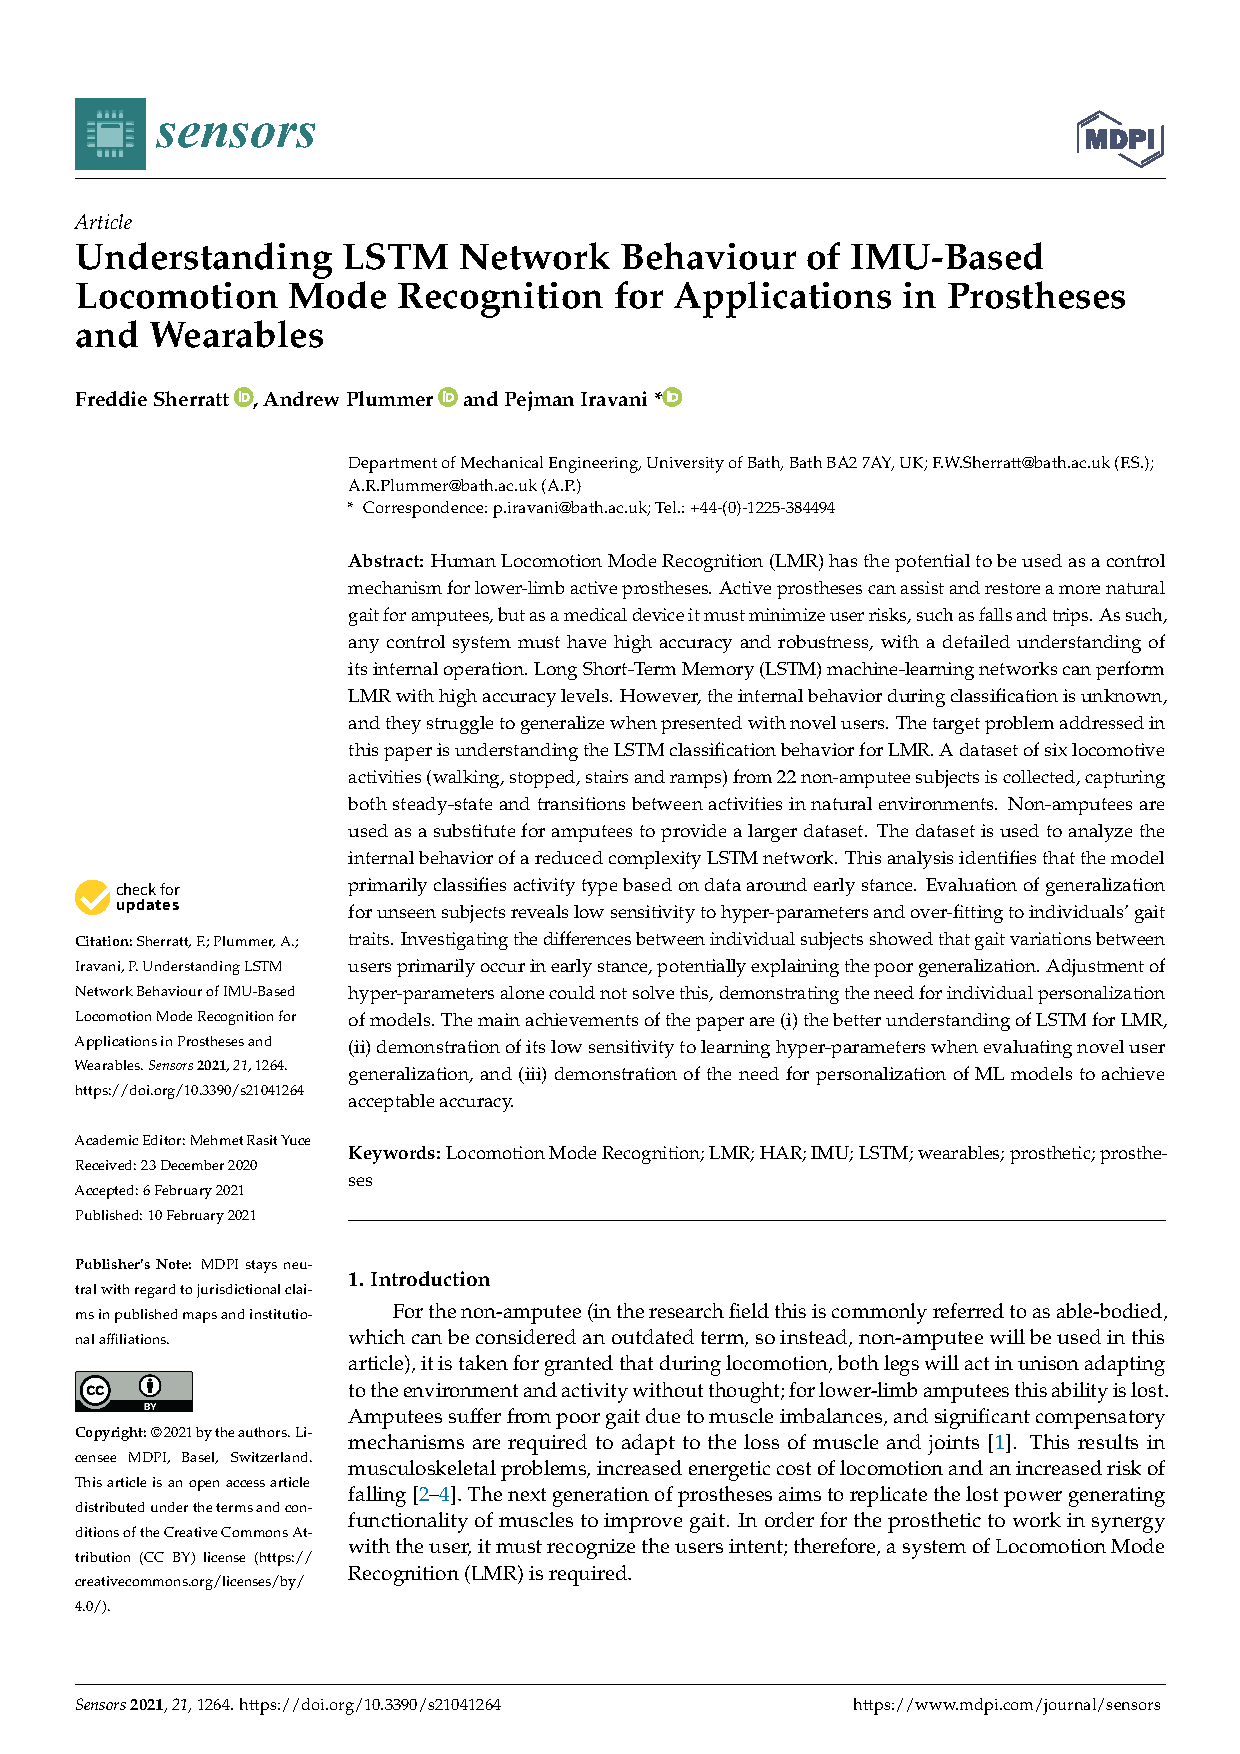
\includepdf[pages=-,scale=.83,offset=11mm 8mm,pagecommand={\thispagestyle{fancy}}, frame=false]{content/4-LSTM_Behaviour/sensors-21-01264-v2.pdf}

% This is a re-typeset of the paper
{\huge\textbf{Understanding LSTM Network Behaviour of IMU-Based Locomotion Mode Recognition for Applications in Prostheses and Wearables}\par}

Freddie Sherratt, Andrew Plummer and Pejman Iravani

Received: 23 December 2020; Accepted: 6 February 2021; Published: 10 February 2021

\textbf{Abstract:} Human \acrfull{lmr} has the potential to be used as a control mechanism for lower-limb active prostheses. Active prostheses can assist and restore a more natural gait for amputees, but as a medical device it must minimize user risks, such as falls and trips. As such, any control system must have high accuracy and robustness, with a detailed understanding of its internal operation. \acrfull{lstm} machine-learning networks can perform \acrshort{lmr} with high accuracy levels. However, the internal behavior during classification is unknown, and they struggle to generalize when presented with novel users. The target problem addressed in this paper is understanding the \acrshort{lstm} classification behavior for \acrshort{lmr}. A dataset of six locomotive activities (walking, stopped, stairs and ramps) from 22 non-amputee subjects is collected, capturing both steady-state and transitions between activities in natural environments. Non-amputees are used as a substitute for amputees to provide a larger dataset. The dataset is used to analyze the internal behavior of a reduced complexity \acrshort{lstm} network. This analysis identifies that the model primarily classifies activity type based on data around early stance. Evaluation of generalization for unseen subjects reveals low sensitivity to hyper-parameters and over-fitting to individuals’ gait traits. Investigating the differences between individual subjects showed that gait variations between users primarily occur in early stance, potentially explaining the poor generalization. Adjustment of hyper-parameters alone could not solve this, demonstrating the need for individual personalization of models. The main achievements of the paper are (i) the better understanding of \acrshort{lstm} for \acrshort{lmr}, (ii) demonstration of its low sensitivity to learning hyper-parameters when evaluating novel user generalization, and (iii) demonstration of the need for personalization of ML models to achieve acceptable accuracy.

\textbf{Keywords}: Locomotion Mode Recognition; LMR; HAR; IMU; LSTM; wearables; prosthetic; prostheses

\section{Introduction}
% Generic introduction to prostheses and the problems users face
For the non-amputee %MFPI: Footnote is not permitted in this journal, so we have moved it into the text, please confirm the whole text. please check all
(in the research field this is commonly referred to as able-bodied, which~can be considered an outdated term, so~instead, non-amputee will be used in this article), it~is taken for granted that during locomotion, both~legs will act in unison adapting to the environment and activity without thought; for lower-limb amputees this ability is lost. Amputees suffer from poor gait due to muscle imbalances, and~significant compensatory mechanisms are required to adapt to the loss of muscle and joints~\cite{Silverman2008}. This~results in musculoskeletal problems, increased energetic cost of locomotion and an increased risk of falling~\cite{Herr2012, Piazza2017, McDonald2018}. The~next generation of prostheses aims to replicate the lost power generating functionality of muscles to improve gait. In~order for the prosthetic to work in synergy with the user, it~must recognize the users intent; therefore, a~system of Locomotion Mode Recognition (LMR) is required.

% What existing solutions are there.
Several commercially available prostheses exist that actively adapt to the user intent, such~as Ottobock's Enpower BiOM~\cite{Enpower}, Blatchford's ElanIC~\cite{ElanIC} and \"Ossur's Proprio Foot~\cite{Proprio}. None~of these three provides more than basic functions, such~as maintaining dorsiflexion during leg swing to increase toe clearance and adjusting ankle resistance based on terrain. Only~the BiOM ankle offers powered assist in push-off, the~controller for this relies on hand-tuned heuristics control strategies~\cite{Montgomery2018}.   {The University of Bath with commercial partners has also been developing a next generastion powered prosthesis}~\cite{Yu2019}.

% Problems\Research gaps
Machine Learning (ML) offers the ability to significantly increase the sophistication of such systems, through understanding of a wide range of activities and personalization to individual characteristics, without specialist intervention~\cite{Labarriere2020}. As~classifying activities is temporal is nature, sequential ML networks, such~as Long Short-Term Memory (LSTM), are~a good fit. LSTM~networks have been demonstrated to be extremely capable at Human Activity Recognition (HAR), accurately identifying actions from locomotive actions, such~as Walking, Running and Stairs~\cite{Murad2017}, to~Hip-Hop dance moves~\cite{Samprita2020}. However, little is known of their understanding internal behavior during these tasks. For~a medical device, such~as a prosthetic, both~a high levels of accuracy and detailed knowledge of internal network operation is required.

% How we are going about answering the research gap/question
This paper explores in detail the operation and performance of LSTM networks for LMR using both seen and novel users. Data~from non-amputee participants is used as a substitute for amputee data as it allows for a much larger and more varied data set while minimizing risk to subjects. This~is then used to investigate the internal operation on a simplified LSTM network. The~effects of hyper-parameters on the generalization performance of a practical LSTM network are then investigated. Finally, changes to the model are investigated to try and improve its performance for novel users. 

% What are the major contributions of this paper
The major contributions of this work are as follows:
\begin{enumerate}
\item Methodology for the collection of a large self-supervised data set of human locomotion data in a natural environment.
\item Provide an insight into the behavior of an LSTM LMR model, and~the performance effects of hyper-parameter selection.
\item Investigation of hyper-parameter sensitivities in an LSTM network and their effect on classification accuracy and generalization to novel user.
\item Demonstration of the need for personalization techniques to account for individual gait traits.
\end{enumerate}

The remainder of this paper is organized as follows; First background theory on the Human Gait Cycle and LSTMs is presented in Section \ref{sec:theory}. Section \ref{sec:related_work} contains Related work followed by Section \ref{sec:materials_and_methdology}---Materials and Methodology, describing the data collection process and setup of the ML environment. The~following Sections  \ref{sec:simplified_model} and \ref{sec:full_complexity}, detail the experiments undertaken, investigating LSTM behavior, and~hyper-parameter sensitivities, respectively. These each follow the same structure with an introduction to the experiment, analysis methodology, then~results and discussions. The~remaining two sections, Sections \ref{sec:discussion} and \ref{sec:conclusion}, contain discussion and conclusions.

\section{Human Gait and Machine-Learning Fundamentals}
\label{sec:theory}
Within this section fundamental theory of the human gait cycle, and~Recurrent Neural Networks (RNN) and LSTMs is presented.

\subsection{Locomotion Mode Recognition and the Human Gait Cycle}

Human gait is a cyclic process that can be delineated by key events. A~gait cycle is defined by two successive Initial Contact (IC) events (the point at which the foot contacts the ground) of the same limb. As~this is normally the heel, it~is often referred to as Heel Strike (HS). Conversely, the~point when the foot leaves the ground is referred to as Toe Off (TO). These two events are used to subdivide the gait into two phases; stance---when the foot is on the ground, and~swing when not. A~diagram showing these events and their location in the gait cycles is shown in Figure~\ref{fig:gait_cycle}.

\begin{figure}[!hbt]
    \centering
    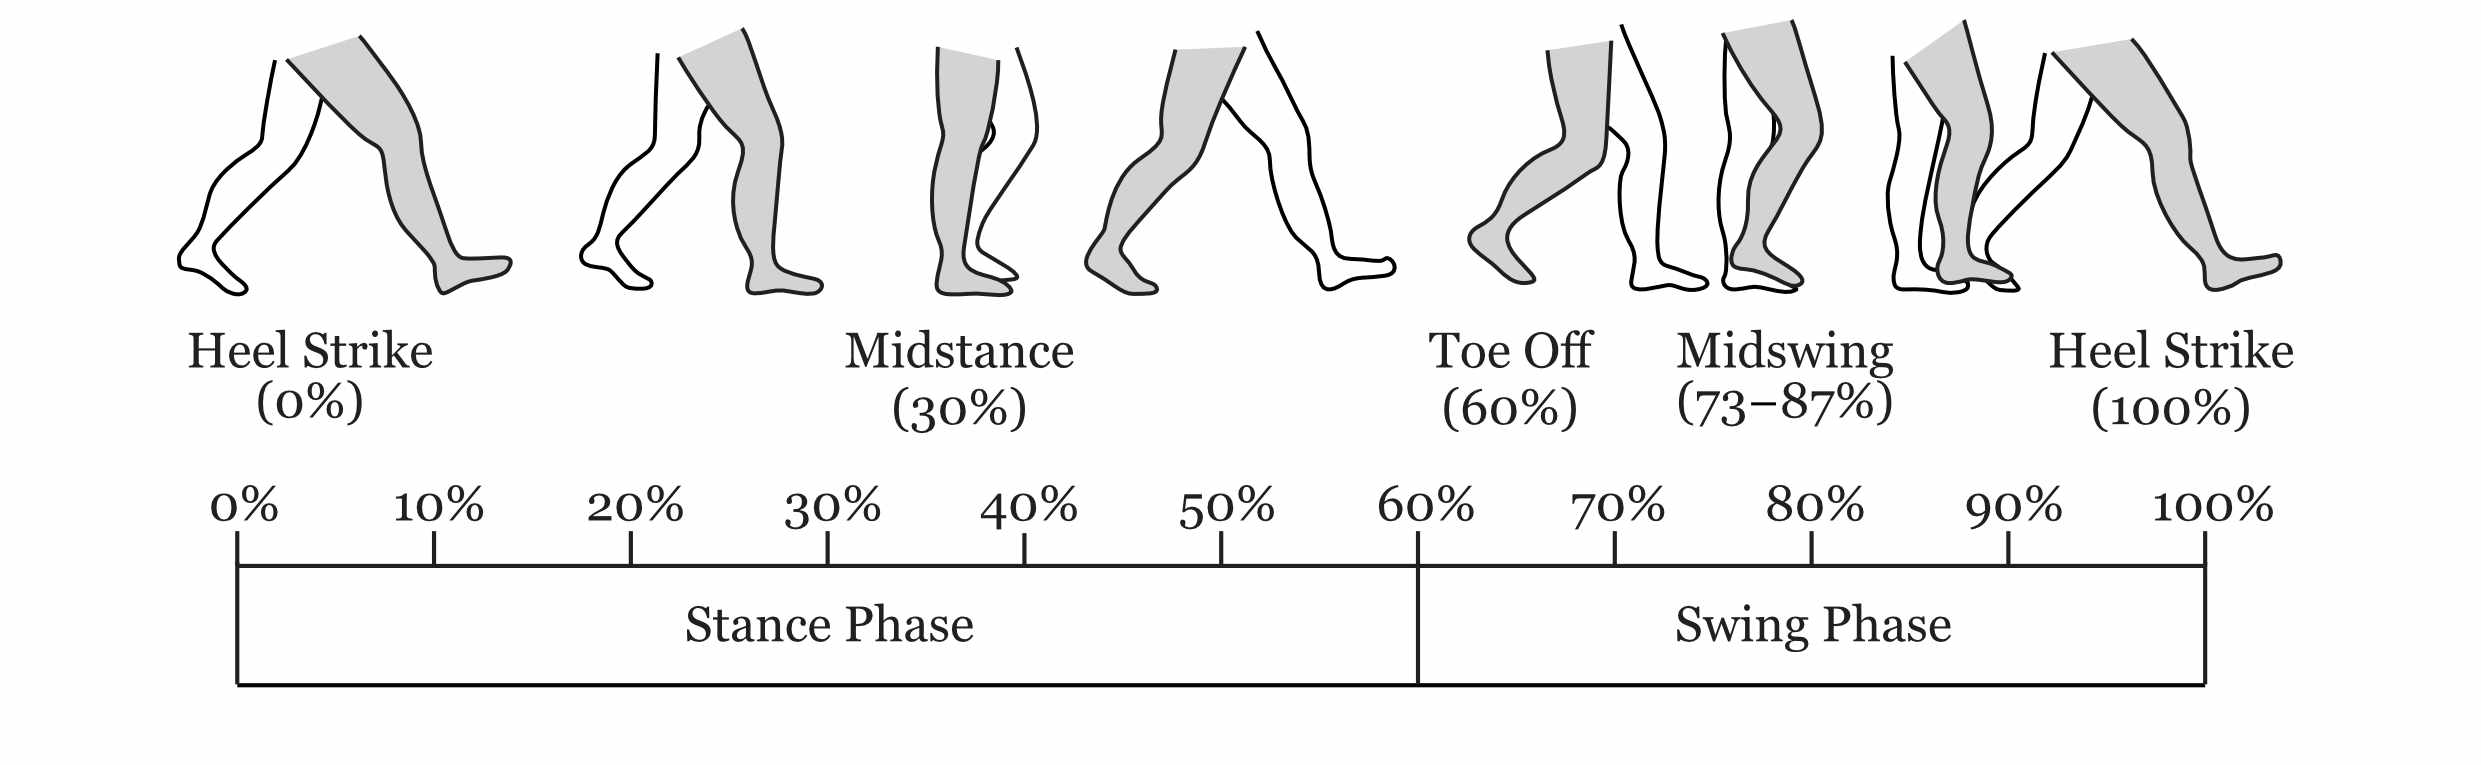
\includegraphics[width=\textwidth]{content/4-LSTM_Behaviour/Gait_Cycle.jpg}
    \caption{Human Gait Cycle during level walking. The~percentage timings of the gait events are approximate, they~vary depending on the individual and environment.}
    \label{fig:gait_cycle}
\end{figure}

It has been shown that gait events can be established from only extrema of the shank angular velocity in the sagittal plane (The sagittal plane divides the body into left and right, so~rotation in this plane is forward and backward motion of the shank) using a technique originally presented by Sabatini et al.~\cite{Sabatini2005}. IC/HS was found to line up with the minima following the peak swing velocity (PK) and TO was identified as the halfway point between the zero-crossing, negative to positive, and~the minima before peak swing. \mbox{Figure~\ref{fig:y-gyro-hs-to}} shows the gyroscope trace of a sensor attached to a subject's shank with the locations of the calculated TO and IC events indicated.

\begin{figure}[!hbt]
    \centering
    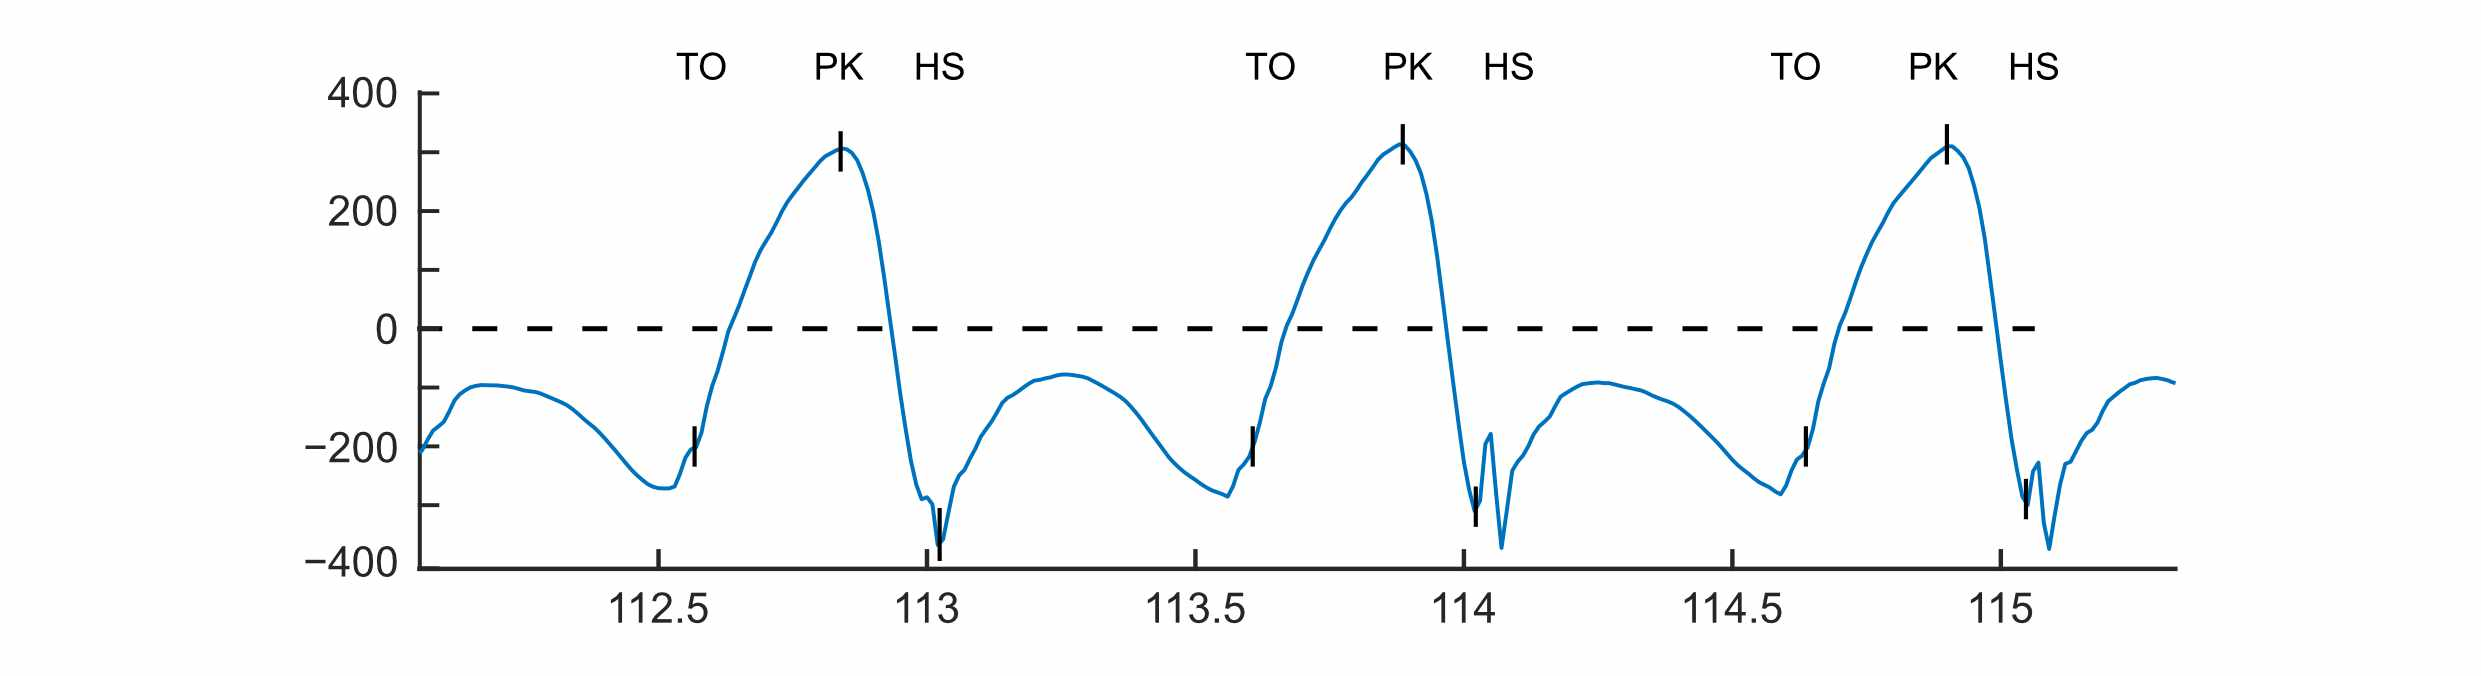
\includegraphics[width=\textwidth]{content/4-LSTM_Behaviour/gyro_trace_hs.jpg}
    \caption{Gait events extracted
 from the sagittal plane gyroscope signal. IC---Initial Contact, PK---Peak Swing, TO---Toe Off.}
    \label{fig:y-gyro-hs-to}
\end{figure}

% How does LMR relate to the human gait?
The action of the leg varies depending on the activity. To~accommodate this, powered prostheses will require multiple locomotive modes to achieve the different timing and power requirements. Therefore, automated recognition of the user's intentions and subsequent selection of the corresponding locomotive mode will be crucial to the performance of devices~\cite{Tucker2015, Windrich2016, Zhang2015}. In~order for amputees to have confidence in a prosthetic device, its~activity recognition must be timely, accurate and consistent and able to account for the individual gait characteristics~\cite{Pedroli2019, Sinha2011, Ponce2016}.

For the current generation of prosthetic devices, this~is achieved through hand-tuned heuristics. These methods identify and associate changing properties of sensor data with different activities. For~example, Coley et al. noted the variation in shank sagittal plane rotational velocity that occur when walking on stairs~\cite{Coley2005}. It~was found that during early stance there is an increase in rotational velocity during stair descent and a decrease during stair ascent when compared to level walking. The~current state of the art in LMR uses ML methods to accomplish activity recognition; these techniques will be discussed further in the next section.

%%%%%%%%%%%%%%%%%%%%%%%%%%%%%%%%%%%%%%%%%%%%%%%%%%%%%%%%%%%%%%%%%%%%%%%%
% Introduce ML in LMR and benefits over heuristics; RNN and LSTM theory; what have other people done in the area
\subsection{Long Short-Term Memory Networks}
\label{sec:lstm_therory}
LMR for active prostheses has conventionally been achieved through heuristic methods with handpicked features that are manually tuned for each individual ~\cite{Maqbool2017, Xu2018}. This approach is favored by the commercial market due to safety and regulatory concerns~\cite{Fluit2020}.  The tuning of these controllers is time-consuming and requires a highly skilled prosthetist. In the current state of the art for LMR techniques, the~focus has been on the use of ML techniques to automate the process of feature selection, output classification, and personalization~\cite{Labarriere2020}.

Many different machine-learning techniques have been investigated including, Support Vector Machines, Hidden Markov Models and Convolution Neural Networks (CNN) with success~\cite{Labarriere2020}. As sensor data from human gait is temporal, the best architecture for solving this will be one that can take into account the sequential nature of the input data. The Recurrent Neural Network (RNN) is an ML architecture suited to handling sequential data as it contains both vertical and horizontal connections. This means that cell activation is related to both the previous time step and the input. Information is therefore passed along the sequence as well as up through layers. Figure~\ref{fig:rnn_structure} shows the unfolded structure of a recurrent network. It can be seen that the activation of each cell is dependent on both its inputs and the hidden states of the previous time steps.

\begin{figure}[!hbt]
    \centering
    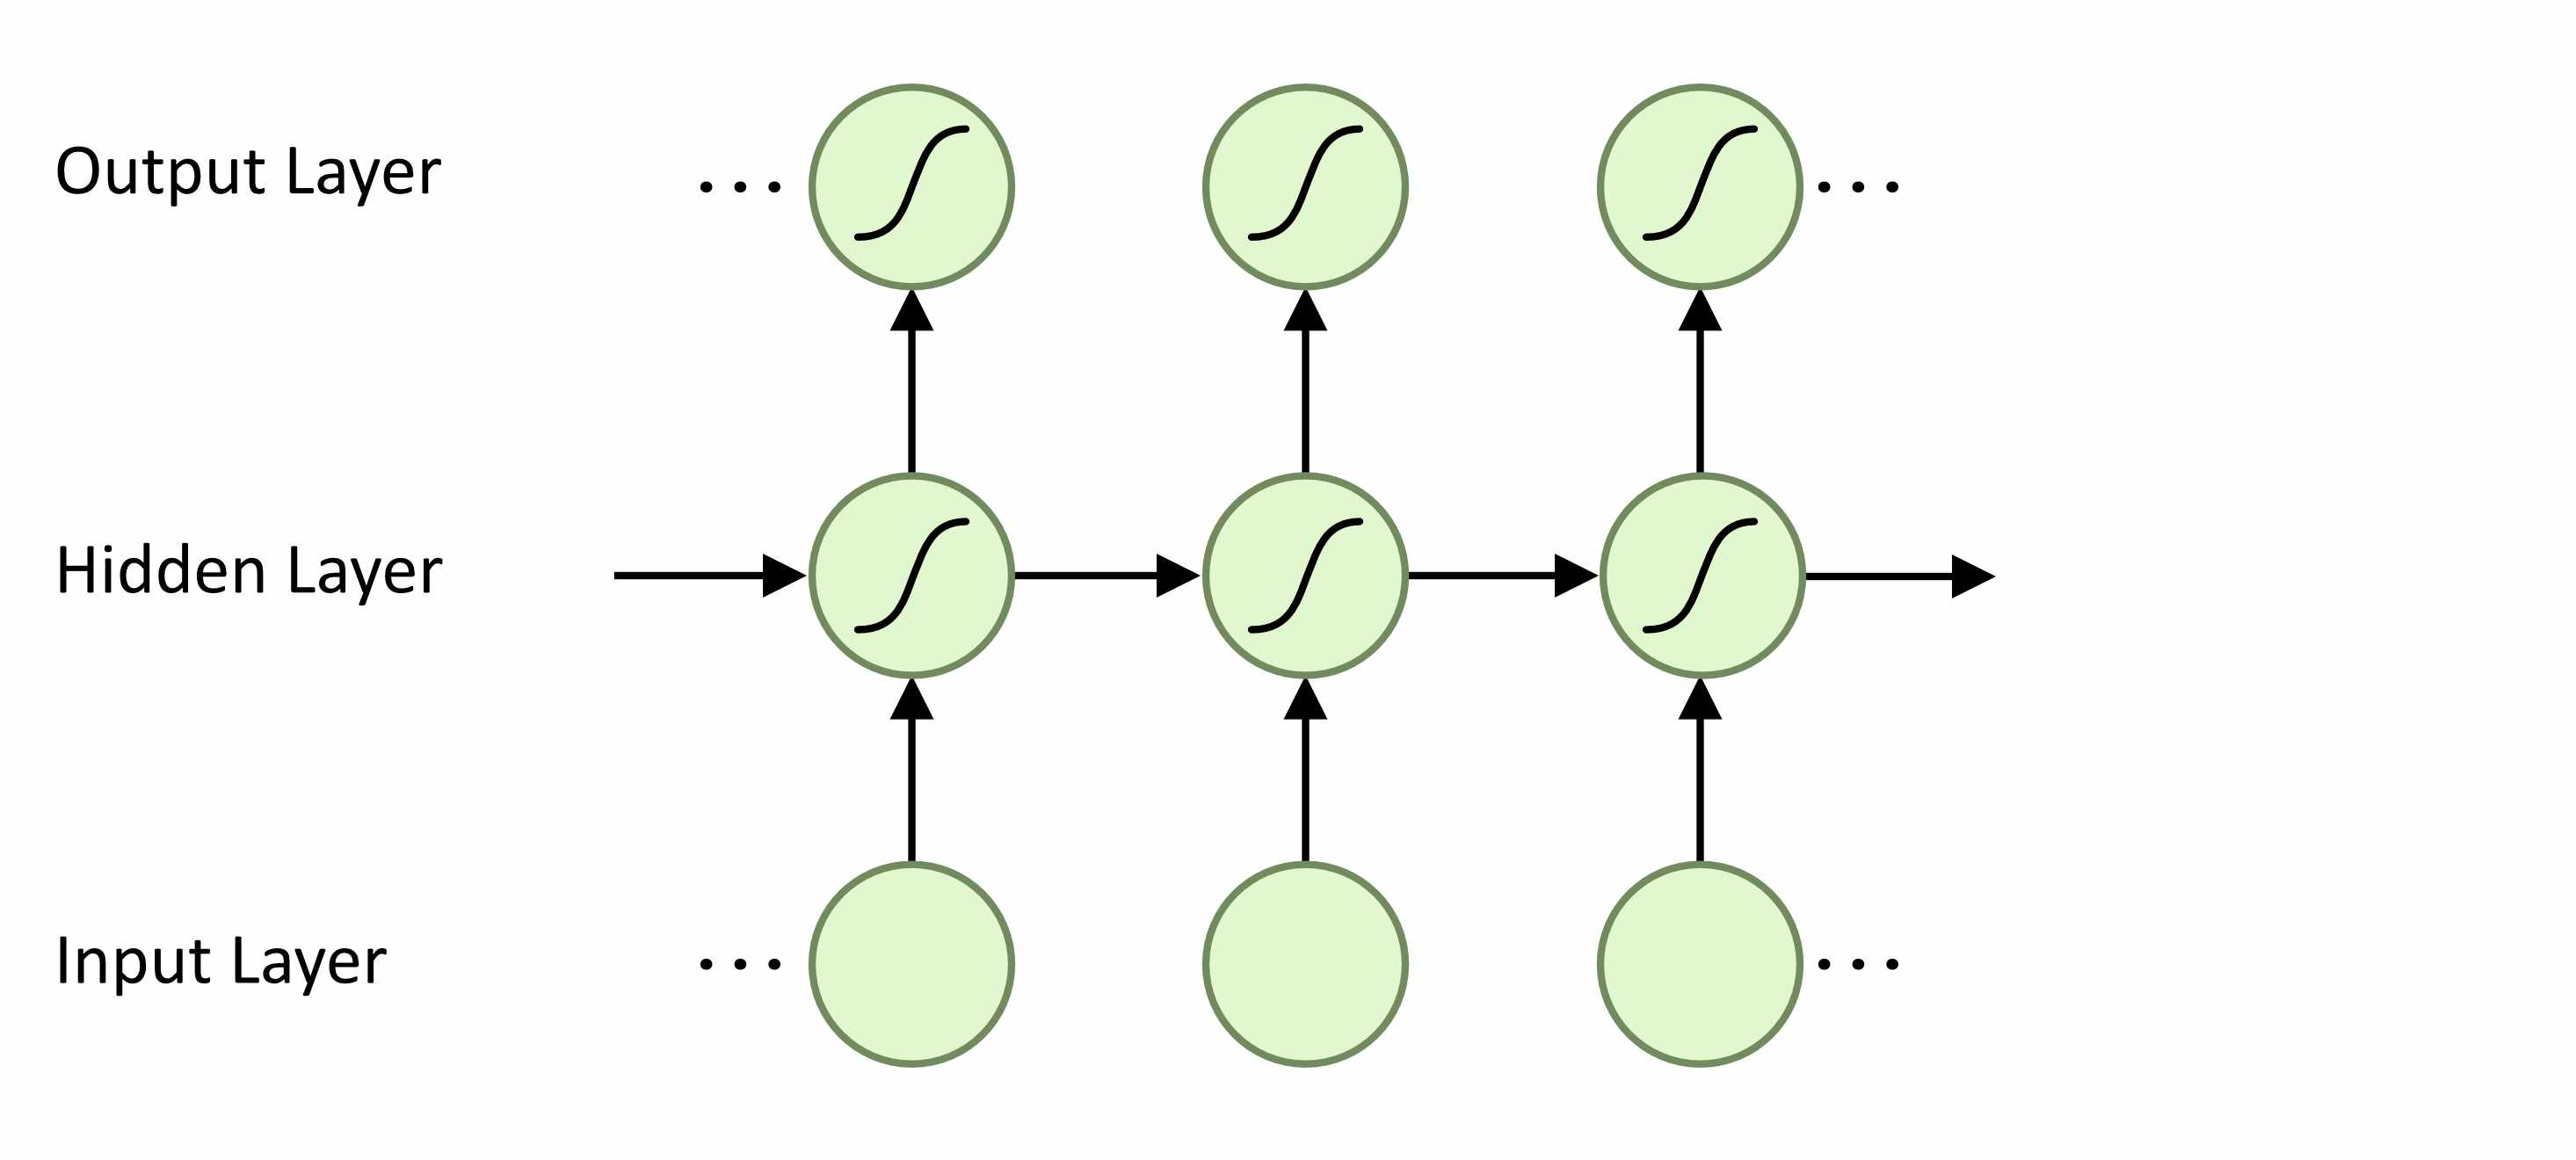
\includegraphics[width=0.7\textwidth]{content/4-LSTM_Behaviour/lstm/rnn_structure.jpg}
    \caption{Unfolded Recurrent Network.}
    \label{fig:rnn_structure}
\end{figure}

Each timestep in the network can contain several hidden states or units. This is represented by Equation (\ref{eqn:rnn_activation}) showing the activation input, $\mathbf{a}^t$. $\mathbf{a}$ is formed from the bias vector $\mathbf{b}$ plus the sum of input vectors $\mathbf{x}$ and previous hidden states $\mathbf{h}$, multiplied by the weight matrices $\mathbf{W}$ and $\mathbf{U}$ for hidden-to-hidden state and input-to-hidden state connections respectively~\cite{Goodfellow2015}. The shape of an RNN network is often described by its timesteps and units, for example, 128 $\times$ 6.

\begin{equation}
    \mathbf{a}^{(t)} = \mathbf{b} + \mathbf{Wh}^{(t-1)} + \mathbf{Ux}^{(t)}
    \label{eqn:rnn_activation}
\end{equation}

%What problems exist with them 
RNNs have been shown to produce good results in some sequential tasks, but~their application is limited by difficulty of training. The primary difficulty is the vanishing/exploding gradient problem. During gradient-based training methods, repeated multiplication by values that are not near one, along long dependency chains results in values that either vanish or explode. A vanishing gradient makes it challenging to know which direction the parameters should move to improve the cost function. Exploding gradients can make learning unstable. Non-gradient-based training has been tried, although to limited success~\cite{Graves2012, Goodfellow2015}.

% LSTM
The Long Short-Term Memory (LSTM) architecture solves the vanishing gradient problem by adding mechanisms for regulating information allowing it to be retained for long periods. Created by Hochreiter and Schmidhuber in 1997~\cite{Hochreiter1997} the LSTM is an RNN style architecture that includes gates to control information flow between cells, see~\mbox{Figure~\ref{fig:lstm_unit}.} Information flowing along the cell state can be modulated by the input and forget gate structures with the final output a filtered version of the cell state based on context from the inputs \cite{Olah2015}.

\begin{figure}[!hbt]
    \centering
    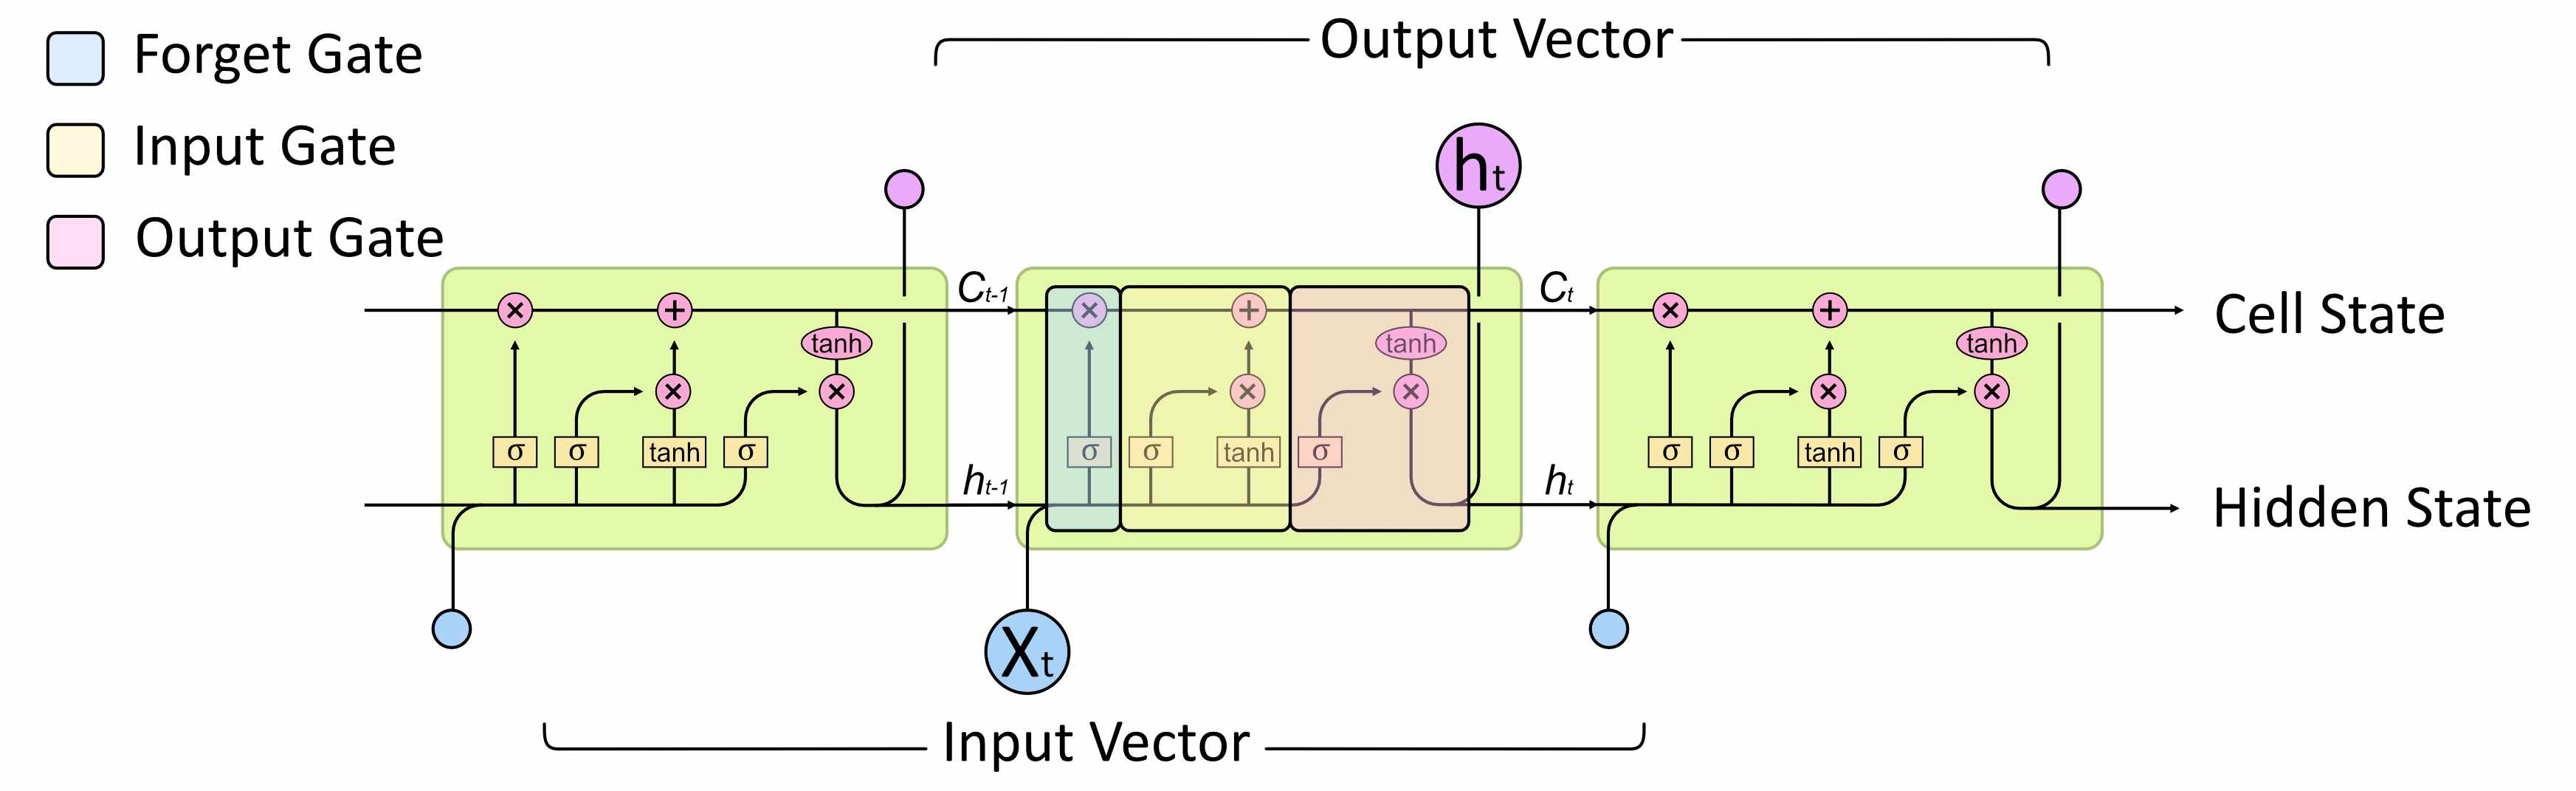
\includegraphics[width=0.9\textwidth]{content/4-LSTM_Behaviour/lstm/lstm_internal_operation.jpg}
    \caption{LSTM unit with input and output connections.}
    \label{fig:lstm_unit}
\end{figure}

\section{Related Works}
\label{sec:related_work}
In HAR tasks, LSTMs have been demonstrated to provide exceptional performance~\cite{Murad2017} although very little work has been done investigating this in the context of prostheses. Labarri\`ere et al. conducted a systematic review of the ML methods used in activity recognition; for assistive device LSTM networks were only used once~\cite{Labarriere2020}.

% Highly performing LSTM networks in LMR - Controlled conditions
LSTM networks have been found to perform highly in HAR and Activities of Daily Living (ADL) tasks. Murad and Pyun investigated Deep LSTM networks for LMR~\cite{Murad2017}. They~trained their network on common ADL datasets, presenting performance in comparison to other ML architectures on the same data sets. The~network they used took raw IMU data as its input, then interpreted the data using four LSTM layers before a late fusion dense layer and a SoftMax classifier were used to produce a class output. The number of units in the LSTM layers was not explicitly stated but appeared to be one. Performance is high achieving 96.7\% accuracy on the UCI-HAD dataset~\cite{Anguita2013} and an improvement on the presented previous classification attempts using CNN, SVM~and other networks. Tufek et al. replicated this result, achieving 93\% accuracy on the UCI-HAD data set using only a three-layer LSTM network~\cite{Tufek2020}.

However, the~accuracy presented is determined from the validation data, a~random 20\% of the source data, so~sufficient separation between training and validation data is not guaranteed. In~the compared work, a~mixture of evaluation techniques is used, most~commonly k-fold cross-validation techniques. With test data selected by leaving out participants~\cite{Koller2018, Sprager2015}. As such, it is not clear that a direct comparison can be made to demonstrate LSTM's superiority.

% Sensor fusion
Different sensor fusion approaches have been tried. Murad et al allowed a deep LSTM network to learn to fuse the sensor modalities~\cite{Murad2017}. Chung et al. used~an ensemble voting arrangement, where each channel modality of sensor data was passed through a separate LSTM network, with a weighted voting system forming the output classification~\cite{Chung2019}. This~achieved a slightly higher accuracy, of~94\%, than~using the sensors individually.

Multiple authors have developed models that use a series of CNN layer first to fuse sensor data from multiple modalities before passing it to a LSTM network~\cite{Abbaspour2020, Ihianle2020, Mutegeki2020, Wang2020, Mekruksavanich2020}. These achieve only minor improvements in performance classification with 95--96\% accuracies. Again, none of the authors were clear about the unit shape of their LSTM networks.

% LSTM network for assistive devices
There are few examples of LSTM networks being used in assistive devices. \mbox{Wang~et al. used~a Deep LSTM network to select locomotion modes for a lower extremity exo-skeleton~\cite{Wang2018}. Five~locomotion modes were classified (sitting, standing, walking and ascending/descending stairs) based on angular information from hip, knee~and ankle joints. A two-layer LSTM network with 128 timestep windows was used.} The hidden states of this were fed into a weighted mean before a SoftMax classifier. Again, the number of units per timestep was not specified. The classifier performed better than the other models tested achieving over 95\%.

% Use of non-amputee subjects as a substitute for amputees
Ben-Yue Su et al. presented work investigating intent prediction for trans-tibial amputees using IMU data and a CNN networks~\cite{Su2019}. Ten~non-amputee and one trans-tibial amputee were asked to perform short walks traversing a short staircase and ramp with a level surface either side. The~non-amputee subjects wore a hands-free crutch to simulate amputation. Three IMUs were attached to the thigh, shank and ankle of the ``healthy'' leg. The CNN classifier identified five steady states and eight transitions between states. An~accuracy of 94\% was achieved by the non-amputee subjects; this dropped to 89\% for the amputee for validation data. When~testing generalization to an unseen user, using Leave One Out Cross-Validation (LOOXV), this~dropped to 82\% for non-amputee subjects. Subject-specific training was recommended. Reasons for poor generalization were not investigated.

% Novel user performance
Research into the generalization of ML HAR Models to new users is limited. Dehghani et al. investigate the metrics used to evaluate the performance of classifiers, particularly regarding their performance on unseen data presented using k-fold cross-validation methods~\cite{Dehghani2019}. The~paper implements various forms of ML, such as Support Vector Machines (SVM) and Hidden Markov Models (HMM) but not LSTM. Dehghani found that using validation data to evaluate performance overestimates accuracy by 10--16\% as the validation data is too similar to the training data. Instead, individual subjects should be excluded and used as test subjects. The~reason for the worse generalization when presented with a novel user has not been investigated.

Investigations into LSTM networks for HAR/LMR have been primarily focused on achieving the highest possible classification accuracy. No~one has investigated the internal operation of the network, or~sensitivities to hyper-parameter selection for these applications. Dehghani et al. identified that model generalization to novel users is an area that also needs further investigation~\cite{Dehghani2019}. This~paper aims to address these areas.

\section{Materials and Methodology}
\label{sec:materials_and_methdology}
To complete the aims of this paper, a~dataset of human locomotion, methods for processing this data and a ML environment are required. This~section details the methodology used to provide this. It~is split into three sections, Sections \ref{sec:data_collection} and \ref{sec:pre-processing} detail the data collection and pre-processing, respectively. Section \ref{sec:machine_Learning} presents the ML environment and methods.

\subsection{Unsupervised Data Collection in Dynamic Natural Environments}
\label{sec:data_collection}
There are several commonly used data sets for LMR of non-amputees. The~OPPORTUNITY activity recognition dataset~\cite{roggan2010} contains 18  classes for Activities of Daily Living (ADL) such as opening/closing doors and drinking from a cup. Each~subject wore seven 6-axis IMUs and 12 3-axis accelerometers while they performed the prescribed actions. The~UCI-HAD dataset~\cite{Anguita2013} recorded subjects performing six activities: walking, stair ascent, stair descent, sitting, standing and lying while wearing a waist-mounted smartphone with onboard Magnetic, Angular Rate and Gravity (MARG) sensors. Both~of these data sets were recorded in controlled conditions, so~do not capture any variation in the activity that may occur due to the environment. Sztyler and Stuckenschmidt collected data from 15~subjects performing eight activities while wearing six wearable sensors. Recording took place in the same natural environments for each activity. Only~steady-state activities were captured and not the transition between them~\cite{Sztyler2017}. Due~to limitation in the identified data sets, a~new set of data is required. 

% Aim of data collection
The aim of the new data set was to record natural locomotion in an unstructured environment, capturing both steady-state and the transition between activities across different settings from a wide range of subjects. Collection of large quantities of data from amputees is very challenging, so~instead non-amputee subjects are used. Non-amputee subjects have a less varied gait than amputees, but~this can be countered by a larger population size.

% Sensor selection and location
Non-invasive wearable sensors, such~as Inertial Measurement Units (IMU), are~an appealing choice for developing such a system. IMUs~give fast update rates, 100s of Hz, are~non-invasive (small with minimal mounting constraints), low~cost and have reasonable accuracy. They~have been widely used in the field, all~of the latest generation of powered prosthetic knees investigated by Fluit et al contained IMUs~\cite{Fluit2020}.

% Which sensors did we use and why
The Suunto Movesense wearable IMU was used to collect activity data. This~is a COTS device containing a nine-axis MARG sensor and a Bluetooth Low Energy (BLE) radio in a small 10~g package. The~sensor housing contains a snap connector allowing it to be clipped on attachment hardware. A~variety of mounting hardware is available off the shelf. The~sensor is user-programmable allowing customized behavior through the Movesense API. To~enable the desired streaming application it was programmed to transmit compressed IMU data at 100Hz over its BLE connection to a custom app running on an android smartphone. The~devices come with Factory calibration for the IMU, no~additional IMU calibration was undertaken.

Five sensors were attached to each participant in the following locations: on the inside of both ankles using an elastic Velcro strap, on~each hip using a clothes/belt clip and across the chest using a heart rate strap. The~location of the sensors was selected to give wide coverage of body movements while providing easy, secure and non-invasive attachment to minimize discomfort and disruption to natural movement. Figure~\ref{fig:movesense_sensors} shows a subject wearing the five sensors.

\begin{figure}[!hbt]
    \centering
    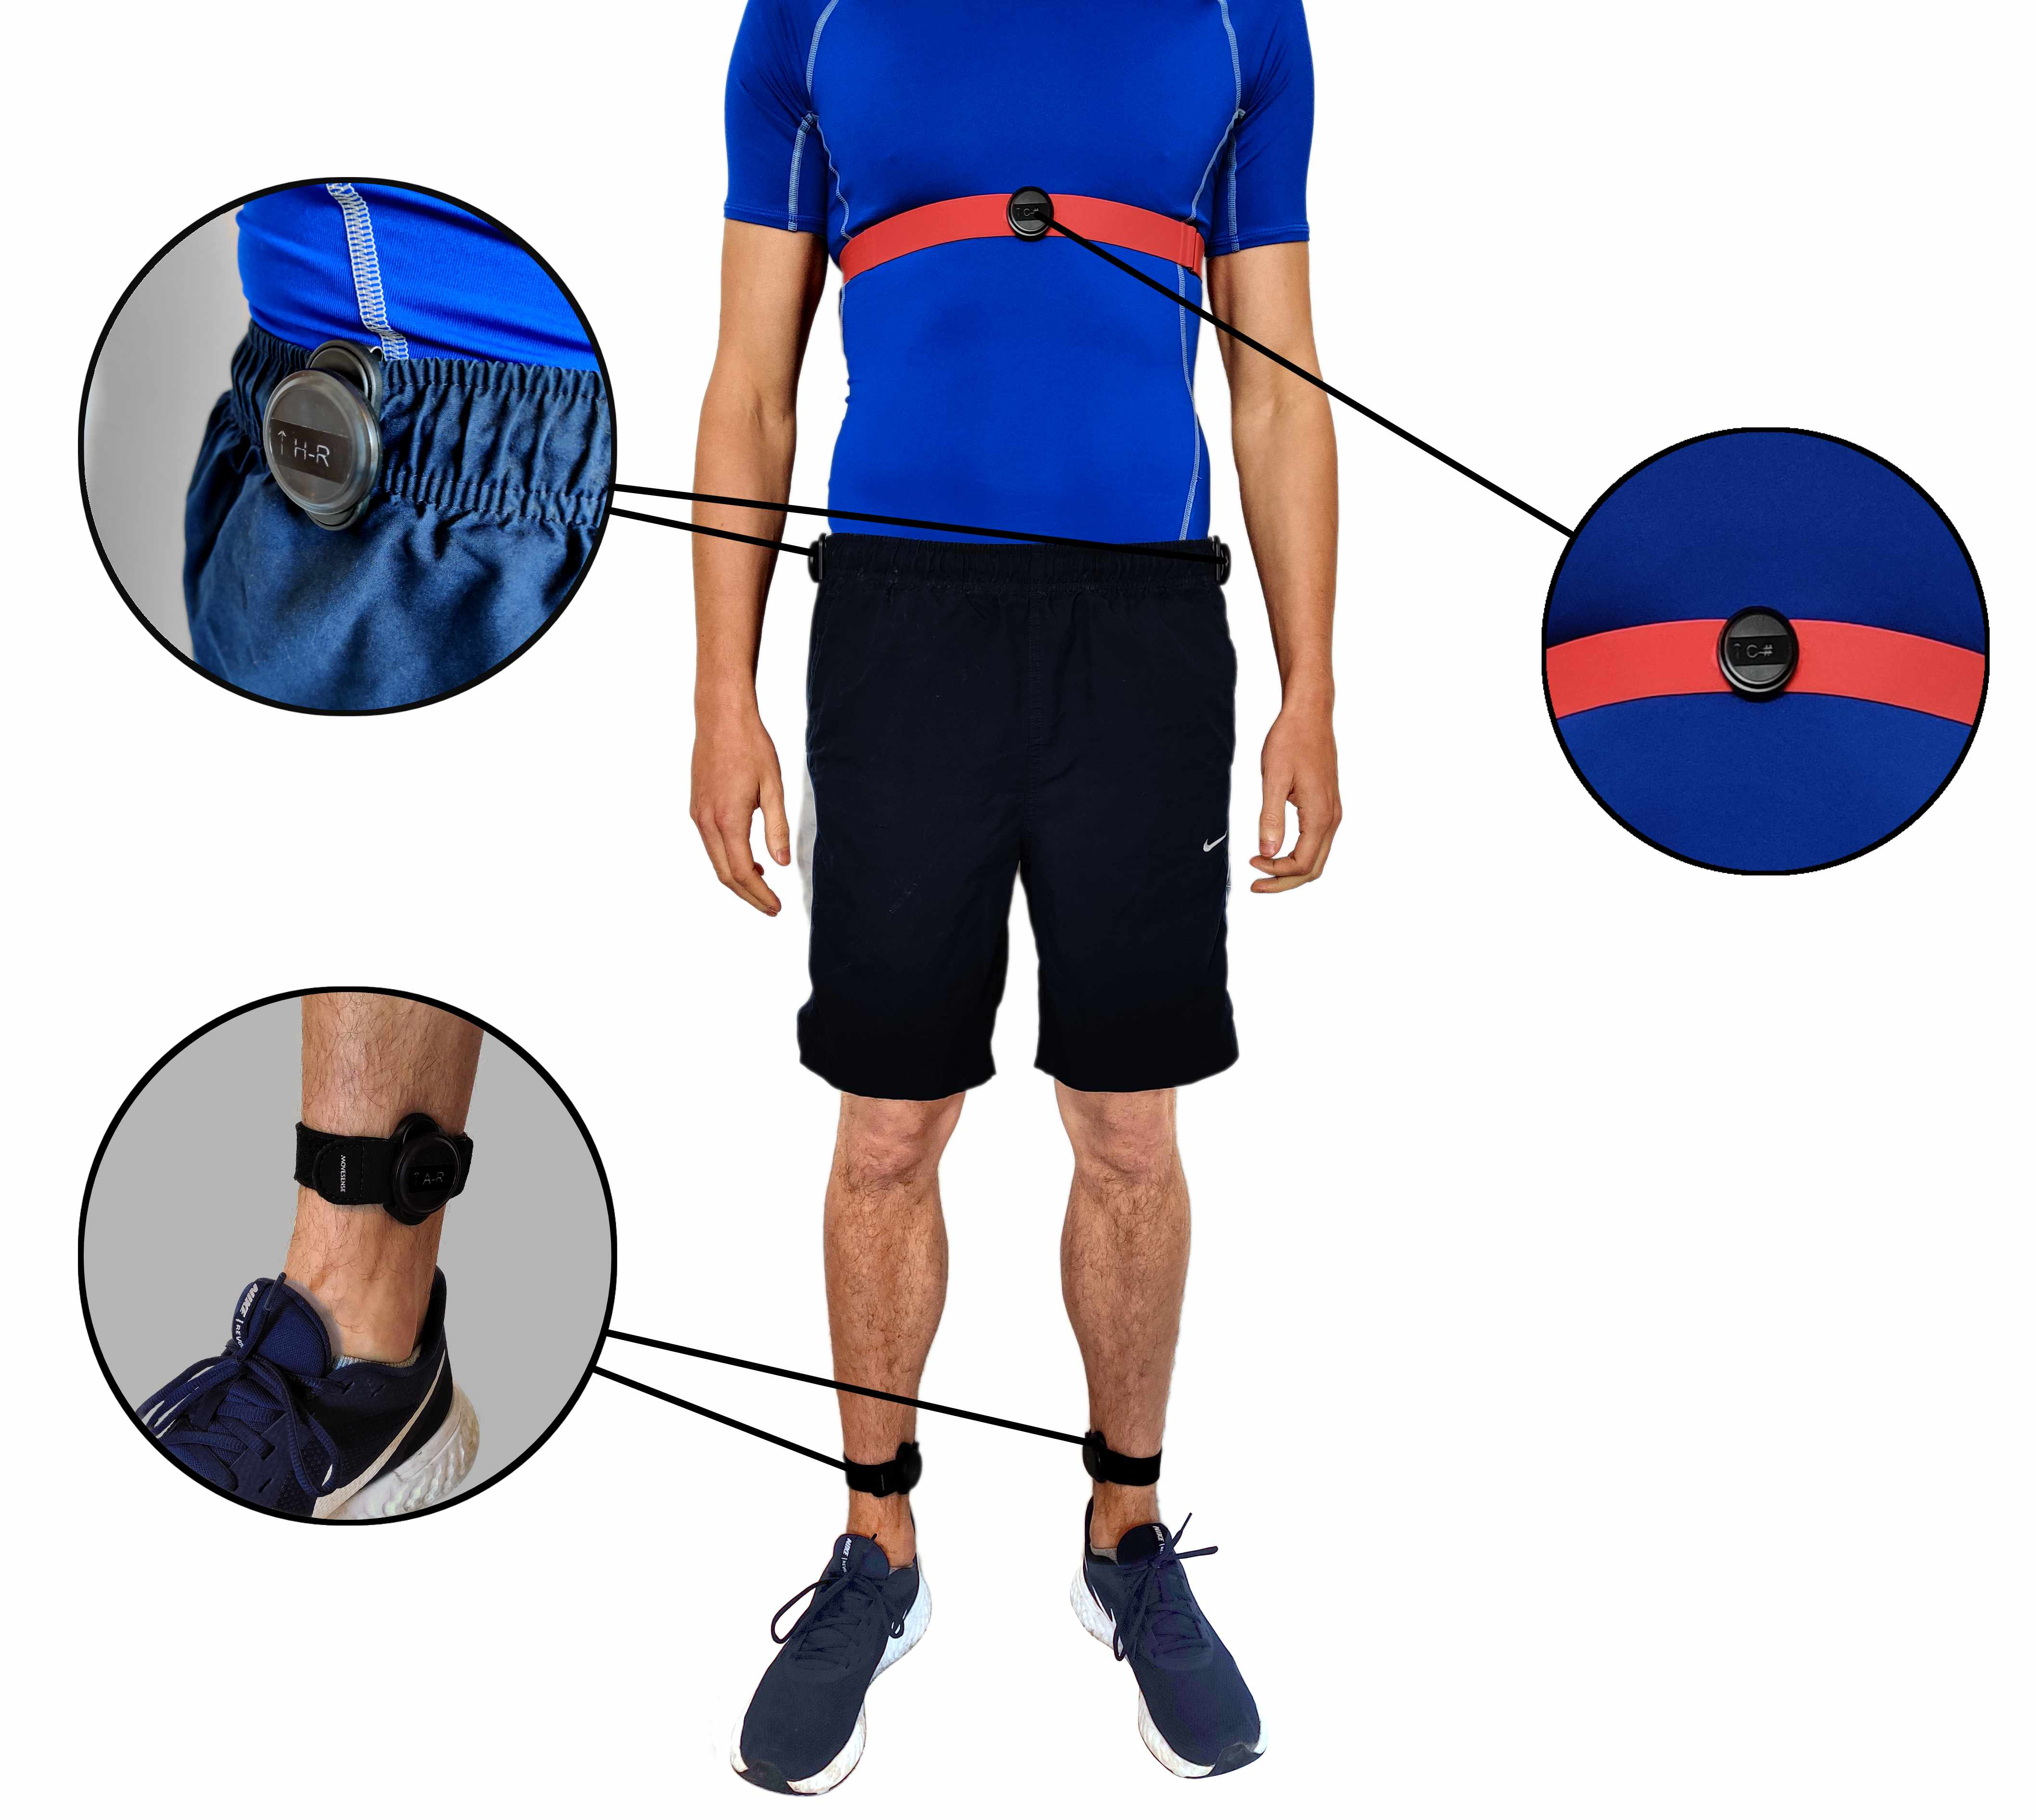
\includegraphics[height=220px]{content/4-LSTM_Behaviour/sensor_locations.jpg}
    \caption{Subject wearing the Movesense IMU sensors on both ankles, hips~and the chest.}
    \label{fig:movesense_sensors}
\end{figure}

To record data from the sensors, a~custom android app was created. This~formed a BLE connection to each device and saved the streamed data. During recording a series of buttons at the bottom of the screen could be used for real-time labelling of activities. Once~recording had finished the subject was presented with an upload screen allowing metadata to be added. The~file could then be shared anonymously with the researchers using Google's Firebase cloud services. A~screenshot of the app in recording mode is shown in Figure~\ref{fig:data_collection_diagrams}.

\begin{figure}[!hbt]
    \centering
    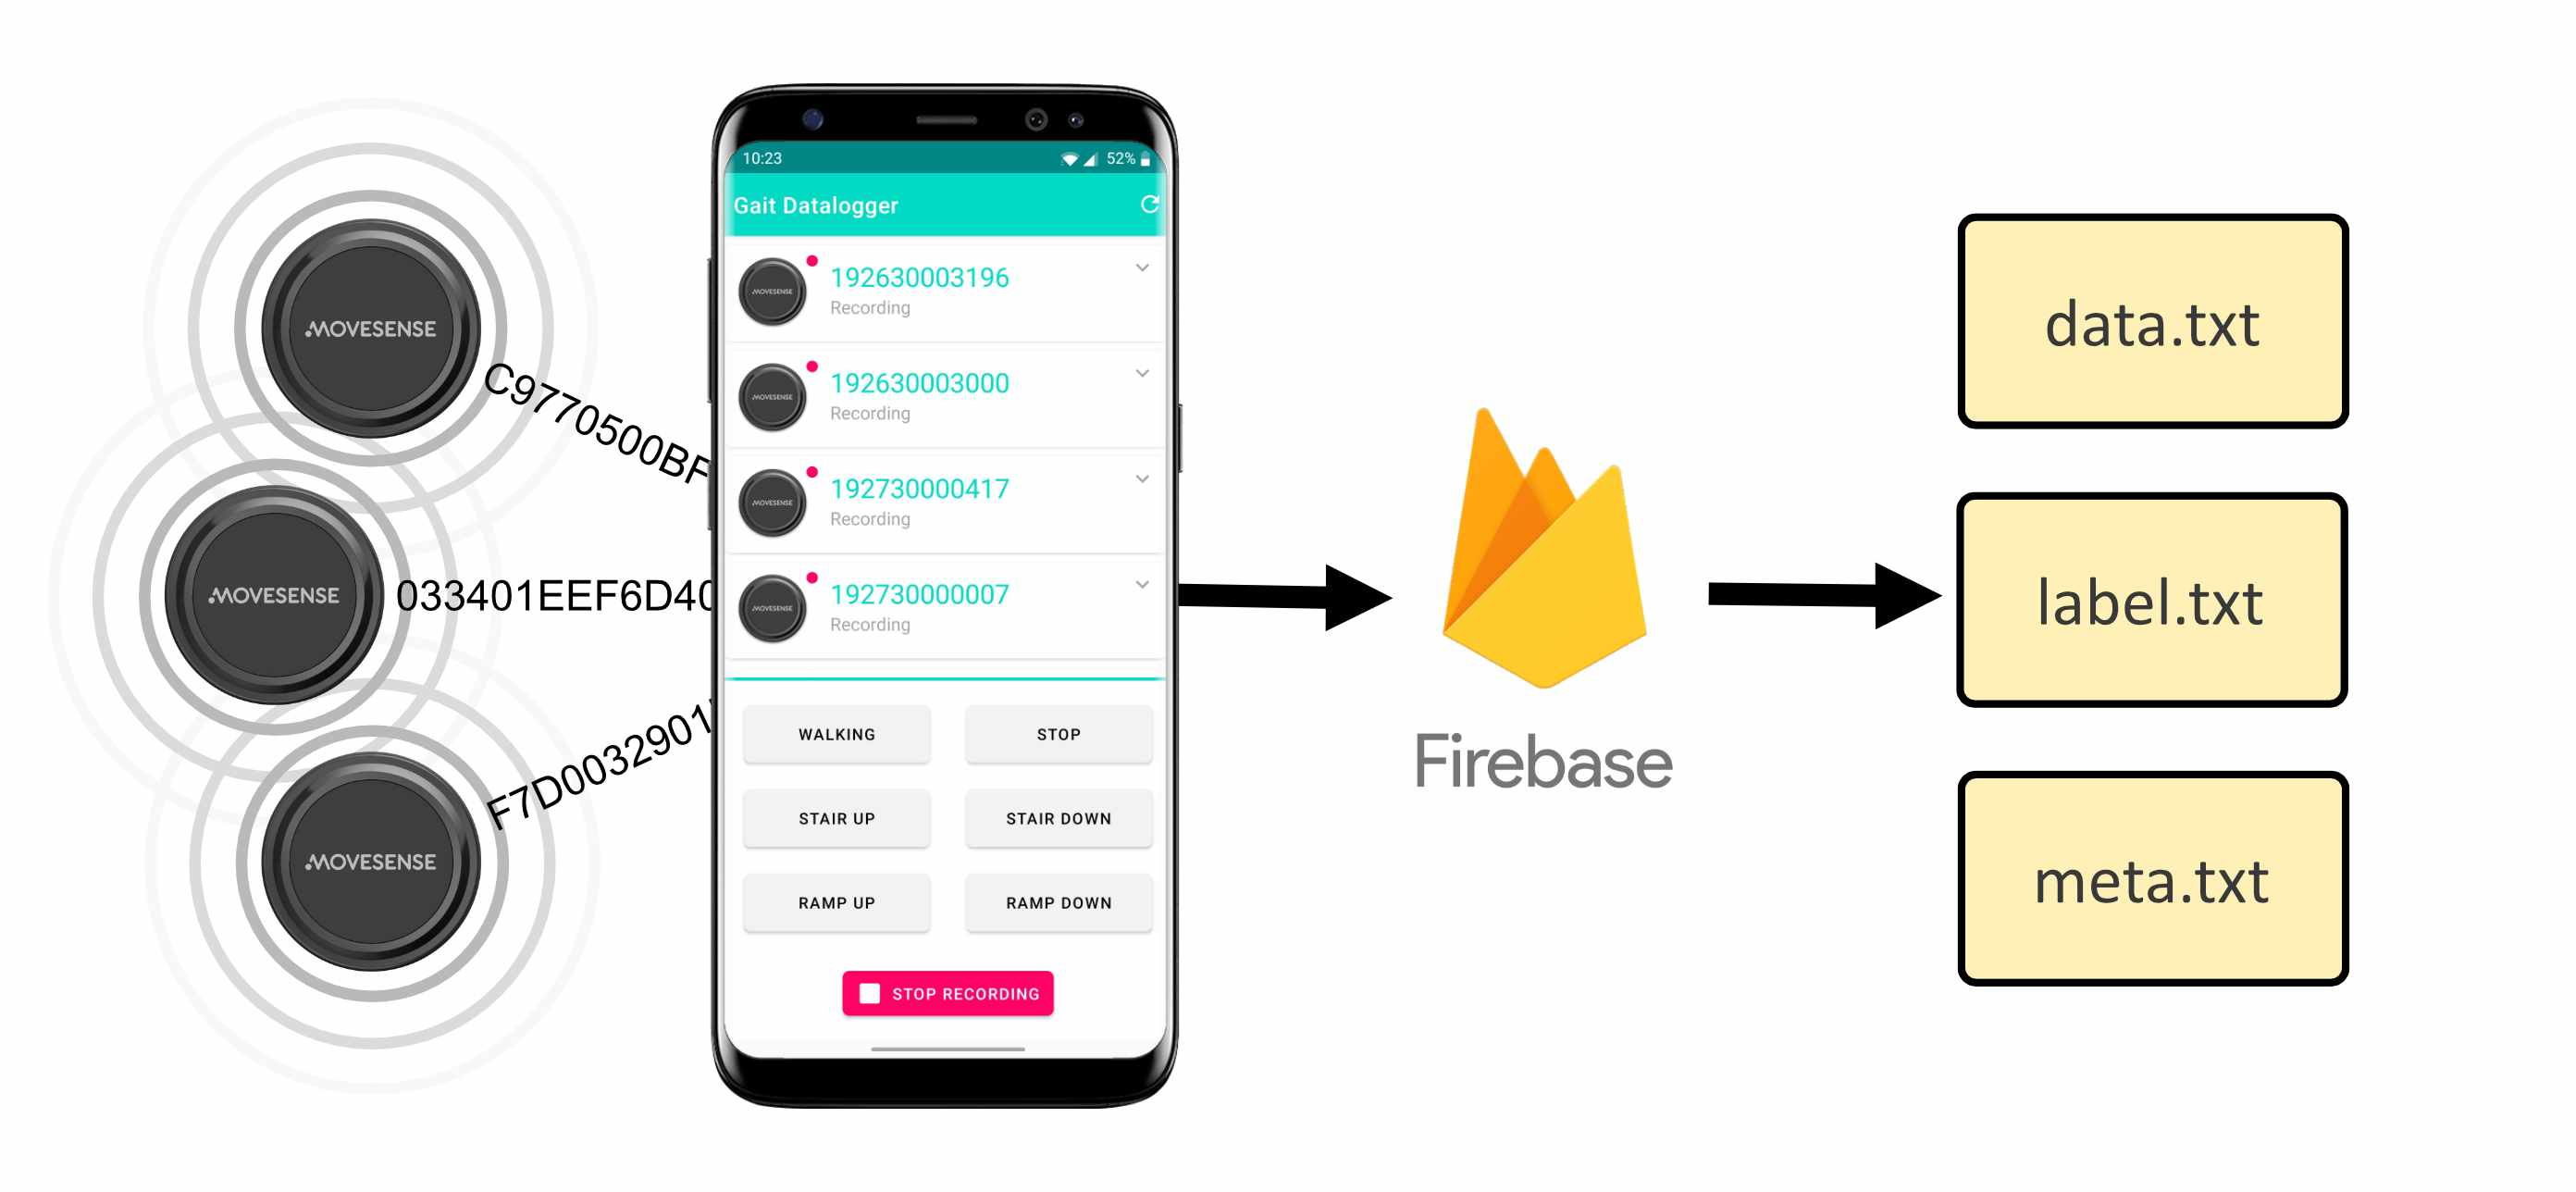
\includegraphics[width=0.8\textwidth]{content/4-LSTM_Behaviour/sensor_collection.jpg}
    \caption{Custom Android app with connected sensors and illustration of Firebase upload system.}
    \label{fig:data_collection_diagrams}
\end{figure}

Study subjects were provided with instructions on how to use the sensing equipment, and~the activity classes, then~allowed to record as they wished. The~following activities were selected, Walking (W), Stair Ascent (SA), Stair Descent (SD), Ramp~Ascent (RA), Ramp~Descent (RD) and Stopped (S). Labarri\`ere et al. identified these as the most commonly investigated and they require no equipment or skill to perform~\cite{Labarriere2020}. The~study received ethical approval from the University of Bath Research Ethics Approval Committee for Health (REACH), reference \textit{EP 19/20 003}.

% Participant instructions
Twenty-two participants of a wide variety of age (mean 29, std~10), gender (17M, 5F), and~physique were chosen to give a broad data set. Participants were instructed to walk around a varied environment with the sensor on while labelling the six activity classes. No~further instructions on how the recording should be conducted were provided. A~total of 268~min  of data was collected, which includes 1170~transitions between activities. Table \ref{tab:data_collected_summary} contains a summary of the data collected. The~number of steps was produced by summing the peak swing gait events for each label.

% % Dataset Statistics
% \begin{specialtable}[H]
%     \centering
%     \caption{Quantity of data collected for each activity.}
%     \label{tab:data_collected_summary}
%     \setlength{\cellWidtha}{\columnwidth/4-2\tabcolsep+0.0in}
% \setlength{\cellWidthb}{\columnwidth/4-2\tabcolsep+0.0in}
% \setlength{\cellWidthc}{\columnwidth/4-2\tabcolsep-0.0in}
% \setlength{\cellWidthd}{\columnwidth/4-2\tabcolsep-0.0in}
% %\setlength{\cellWidthe}{\columnwidth/8-2\tabcolsep-0.0in}
% %\setlength{\cellWidthf}{\columnwidth/8-2\tabcolsep-0.0in}
% %\setlength{\cellWidthg}{\columnwidth/8-2\tabcolsep-0in}
% %\setlength{\cellWidthh}{\columnwidth/8-2\tabcolsep-0in}%
% \scalebox{1}[1]{\begin{tabularx}{\columnwidth}{>{\PreserveBackslash\centering}m{\cellWidtha}>{\PreserveBackslash\centering}m{\cellWidthb}>{\PreserveBackslash\centering}m{\cellWidthc}>{\PreserveBackslash\centering}m{\cellWidthd}}
% \toprule
%         \textbf{Activity} & \textbf{Samples} & \textbf{Time (min)} & \textbf{Number of Steps} \\
%          \midrule
%          Walking & 1,075,211 & 179 & 9438 \\
%          Stair Ascent & 139,922 & 23 & 1286 \\
%          Stair Descent & 122,379 & 20 & 1280 \\ 
%          Ramp Ascent & 73,328 & 12 & 656 \\
%          Ramp Descent & 79,436 & 13 & 754 \\
%          Stop & 121,027 & 20 & - \\
%          \midrule
%          \textbf{Total} & 1,611,303 & 268 & 13,414\\
%           \bottomrule
% \end{tabularx}}
% \end{specialtable}
\begin{table}[!hbt]
    \centering
    \caption{Quantity of data collected for each activity.}
    \label{tab:data_collected_summary}
    \begin{tabularx}{\textwidth}{YYYY}
        \textbf{Activity} & \textbf{Samples} & \textbf{Time (min)} & \textbf{Number of Steps} \\
        \hline
        Walking & 1075211 & 179 & 9438 \\
        Stair Ascent & 139922 & 23 & 1286 \\
        Stair Descent & 122379 & 20 & 1280 \\ 
        Ramp Ascent & 73328 & 12 & 656 \\
        Ramp Descent & 79436 & 13 & 754 \\
        Stop & 121027 & 20 & - \\
        \hline
        \textbf{Total} & 1611303 & 268 & 13414
    \end{tabularx}
\end{table}
\clearpage


\section{Post-commentary}
Since being published, seventeen papers have cited the article\footnote{as of the 23\textsuperscript{rd} July 2022}. A number of these citations have used the paper as an example use case for an \acrshort{lstm} network\cite{Uddin2021, Du2021, Velezguerrero2021, Low2022, Bittibssi2022} and data capture methods\cite{Shin2021, Su2021}. The paper was also awarded a Editor's Choice award. The award is given to articles the journal editors believe are of particularly interesting or important in a field.

Maximum performance for validation data was 96.1\% . This classification accuracy is comparable in performance with literature. Uddin et al.~achieved 94\%\cite{Uddin2021} and Murad et al.~achieved 97\%\cite{Murad2017}. However the performance of the test set, containing novel unseen individuals, was significantly lower at 76\%. 

This results supports the conclusion drawn by Dehghani et al. that a substantial drop in performance for unseen subjects is to be expected\cite{Dehghani2019}. This work extends on that conclusion by proposing that the high variability between individuals during early stance is a large source of this error. As when the target user behaviour differs from the training dataset the subject will perform poorly\cite{Qiu2022}. 

Therefore for a general model to perform well the training set would need to include individuals with a similar gait pattern to all target subjects. This is highly impractical especially for amputee who have significantly more variability in their gait\cite{Lechler2018, Kovac2009}. It is also harder to get data for amputees due to reduced mobility therefore harder to add them into the general training pool\cite{Gardiner2016}.

% What was the big takeaway from this paper - demonstrates the need for personalisation
The paper's outcomes expressed the need to adapt the trained model to each target individual through a method of personalisation in order to perform adequately. It also noted the need for additional testing to demonstrate the suitability of these techniques for amputees. These needs will be explored further in the subsequent chapters.

